%!TEX TS-program = pdflatex
%!TEX root = i3det-top.tex
%!TEX encoding = UTF-8 Unicode

\section{\label{sect:online}Online Systems}
\textsl{(John K; 12-15 pages)}

The IceCube online systems comprise both the software and hardware
at the detector site responsible for data acquisition, event selection,
monitoring, and data storage and movement.  As one of the goals of IceCube
operations is to maximize the fraction of time the detector is sensitive
to neutrino interactions (``uptime''), the online systems are modular so
that failures in one
particular component do not necessarily prevent the continuation of basic
data acquisition. Additionally, all systems are monitored with a combination of
custom-designed and industry-standard tools so that detector operators can
be alerted in case of abnormal conditions.

\subsection{\label{sect:online:dataflow}Data Flow Overview}

The online data flow consists of a number of steps of data reduction and
selection in the progression from photon detection in the glacial ice to
candidate neutrino event selection, along with associated secondary data
streams and monitoring.  An overview of the data flow is shown in
Fig.~\ref{fig:dataflow}.

\begin{figure}[!h]
 \centering
 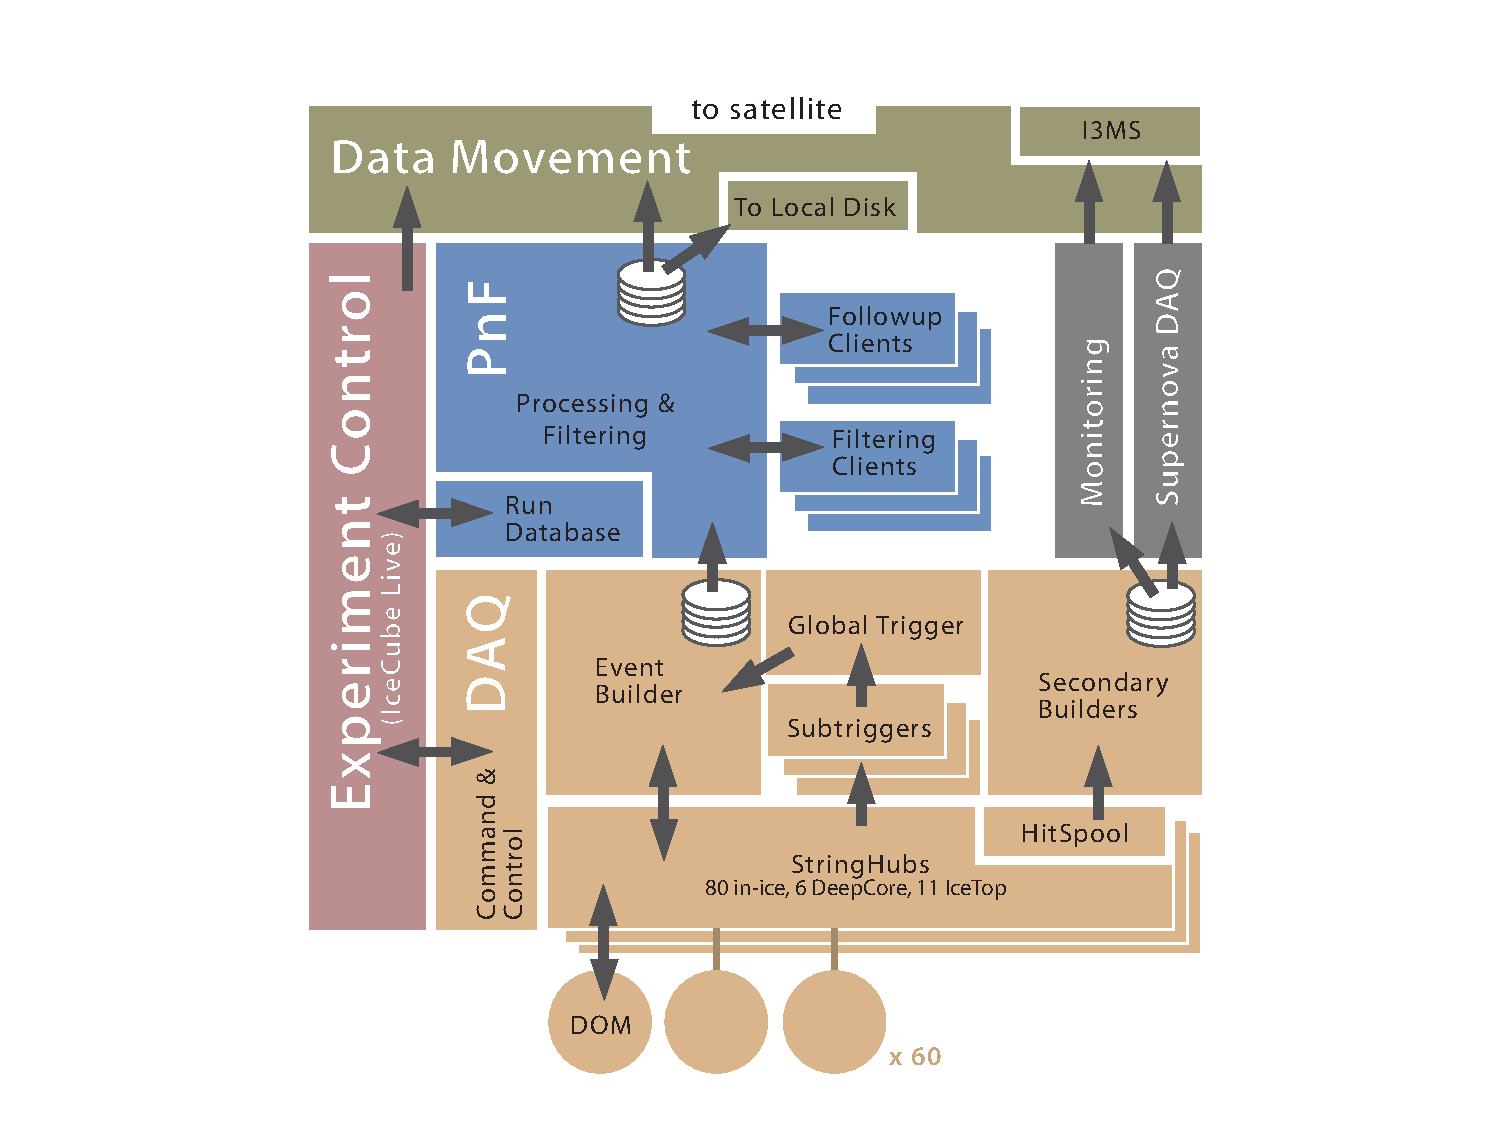
\includegraphics[width=0.6\textwidth]{graphics/online/online_dataflow.pdf}
 \caption{Data flow in the primary IceCube online systems.}
 \label{fig:online_dataflow}
\end{figure}

Since the majority of photons detected by the DOMs are dark noise, a
first-level \emph{local coincidence} (LC) is formed between neighboring
DOMs deployed along the same cable, using dedicated wire pairs within the
in-ice cable.  DOM-level triggers, or \emph{hits}, with corresponding
neighbor hits are flagged with the LC condition (HLC hits), while hits without the
condition (SLC hits) are compressed more aggressively.  The LC time window
as well as the span of neighbor DOMs up and down the cable can both be configured,
with standard settings of a $\pm1 \mu s$ coincidence window and neighbor
span of 2 DOMs.

All DOM hits are read out to dedicated computers on the surface by the data
acquisition system (DAQ).  The next level of data selection is the
formation of \emph{triggers} by the DAQ system.  LC-flagged hits across the
detector are examined for temporal and in some cases spatial patterns that
suggest a common causal relationship.  A number of different trigger
algorithms run in parallel, described in Sect.~\ref{sect:online:trigger}.  All hits
(both LC-flagged and non-LC hits) within a window around the trigger are
combined into \emph{events}, the fundamental output of the DAQ, and written
to disk.  The event rate is approximately 2.5 kHz but varies with the
seasonal atmopheric muon flux, and the total DAQ data rate is approximately
1TB/day.

The DAQ also produces \emph{secondary streams} that include time
calibration, monitoring, and DOM scaler data.  The scaler data, which is
monitoring the noise rate of each DOM in 1.6 ms bins, is used in the
supernova data acquisition system \cite{IC3:supernova} to detect a global rise from
many $O(10)$ MeV neutrino interactions occuring in the ice from a
Galactic core-collapse supernova.  The time calibration and monitoring
streams are used to monitor the health and quality of the data-taking runs.

The raw DAQ event data is then processed further with a number of
\emph{filters} in order to select a subset of events (less than 10\%) to
transfer over satellite to the Northern Hemisphere (see
Sect.~\ref{sect:online:filter}).  Each
filter, typically designed to select events useful for a particular physics
analysis, is run
over all events using a computing cluster in the IceCube Lab.  Because of
limitations both on total computing power and bounds on the processing time
of each event, only fast directional and energy reconstructions are used.
The processing and filtering (PnF) system is also responsible for applying
up-to-date calibrations to the DAQ data; processed events, even those not
selected by the online filters, are stored locally for archival.

A dedicated system for data movement handles the local archival storage to
tape or disk, as well as the handoff of satellite data (see Sect.~\ref{sect:online:jade}).
This includes not only primary data streams but also monitoring data,
calibration runs, and other data streams.

Experiment control and detector monitoring are handled by IceCube Live.
LiveControl interfaces with online software components and provides a
command-line and web interface to each of them, along with higher-level
operations such as starting or stopping runs, setting special run modes for
commissioining and calibration data, and specifying detector
configurations.  The web site component, LiveView, runs both in the ICL and
in the Northern Hemisphere, and provides a near-real-time view of detector
health.  

%An overview of the data flow from DOMs to the satellite.  Description of
%architecture and levels of data reduction, starting with a review of LC and
%proceeding to triggers and then filters.  Secondary streams and SNDAQ.
%I3Live, experiment control, and monitoring.

%The division between \textit{triggering} and
%\textit{filtering} is the urgency of the processing.
%Triggers must operate within a bounded time or
%data is lost.  Filters operate behind such large buffers
%that this is not a consideration.  Historically this means
%that the triggers have been rather \emph{dumb} but there
%is in principle no ceiling to the trigger complexity.

\subsection{\label{sect:sps}SPS and SPTS}

The South Pole System (SPS) comprises 18 racks of computing and
network hardware in the ICL that run the various online systems described in this
section.  The DOM surface cables are connected via passive patch panels to
custom 4U DOMHub computers, one DOMHub per in-ice string and 11 additional
hubs for IceTop.  The remaining servers, including those for higher-level
data acquisition, event filtering, detector monitoring, and core
infrastructure, are currently 2U Dell PowerEdge R720 servers (see Table
\ref{tab:sps_breakdown}).  The servers are typically upgraded every 3 to 4
years.  The custom hardware components in the DOMHubs are replaced with spares as
failures warrant, and the disks and single-board computer (SBC) were
upgraded in 2013--14.

\begin{table}[h]
  \centering
  \begin{tabular}{ r | c }
    \bf{Component} & \bf{\#} \\
    \hline
    DOMHubs & 97 \\
    Data acquisition & 4 \\   
    Event filtering & 23 \\
    Monitoring & 3 \\
    Infrastructure & 7 \\
  \end{tabular}
  \caption{Breakdown of computing equipment at SPS, indicating number of
    machines used for each task. CHECK NUMBERS} 
  \label{tab:sps_breakdown}
\end{table}

The DOMHub is an industrial computer chassis with custom components for
DOM power, timing, and communication.  A low-power single-board computer
communicates with 8 custom PCI DOM Readout (DOR) cards via a backplane.  A
dual-redundant ATX power supply powers the DOMHub, while two 48V Acopian
power supplies, mounted and connected in series inside the chassis, supply
power to the DOMs.  The DOM power is switched and monitoring by the DOR
cards and is controllable by software.  Another PCI card, the DOMHub
Service Board (DSB), is responsible for GPS timing fanout (see
Sect.~\ref{sect:online:master_clock}).

Include Fig.7 from DOM/DAQ paper (hub diagram)?

The SPS computers are connected via a 48 Gbps switch that in turn fans out
to switches in each DOMHub rack; the DOMHub switches are connected with
dual bonded 10 Gbps links.  The hubs and servers are connected to local
switches with dual bonded 1 Gpbs links.  Typical network I/O during data-taking for the
DAQ event builder (see Sect.~\ref{sect:online:evbuilder}) is $\sim30$ MBps in each
direction, while the master PnF node sees 25 MBps in and 80 MBps out.

Redundancy and continuous monitoring of SPS is one of the keys to a high
detector livetime.  Nagios monitoring software detects and flags problems,
including issues with DOM power and communication on the hubs.  Severe
problems impacting data-taking result in a page to the IceCube
winterover personnel via the station's Land Moble Radio (LMR) system. 
A dedicated hot spare server can replace any failed DAQ
node, while spare PnF filtering clients can be started to increase
throughput in case of a data filtering backlog.  SPS hardware is also
connected to dual redundant uninterruptible power supplies 
(UPS) in order to continue data-taking through station power outages of up
to 15 minutes.  

A scaled-down version of SPS, the South Pole Test System (SPTS), allows
testing and validation of both hardware and software in the Northern
Hemisphere before rollout to SPS.  Servers and DOMHubs identical to those
at SPS, along with a small number of DOMs in chest freezers, are used in
the test system.  Although the number of DOMs available is much smaller
than in the real detector, recent software improvements have allowed the
``replay'' of pre-recorded raw SPS hit data on SPTS systems, providing a data stream to
higher-level DAQ and PnF components identical to SPS.

\subsection{Data Readout and Timing}

While the low-level communications and timing systems of the DOM are
described in detail in Ref.~\cite{ref:domdaq}, we review those here in the
context of the broader online systems.

\subsubsection{\label{sect:online:comms}Communications}

Digital communication between the DOR card and DOM occurs via copper
twisted pairs, with two DOMs per pair on the in-ice cable, and one IceTop
DOM per pair for increased bandwidth.  The physical
layer signaling is via amplitude shift key (ASK) modulation.  The protocol
is a custom packet-based scheme.  Each packet is assigned a sequence 
number, and all received packets are acknowledged if the sequence number is
correct.  Each packet also contains a CRC checksum to detect transmission
errors.  Out-of-sequence packets received are ignored, and non-acknowledged
packets are retransmitted.  

Messaging is managed from the surface, in that the DOR requests data
from each DOM in turn; only one DOM can transmit at a time.  Communication
is stopped every second to perform a timing calibration (RAPCal) via
reciprocal bimodal pulse transmission \cite{ref:domdaq}; this provides a
time-dependent translation of DOM clock to DOR clock for every module.  The
total bandwidth of the communication channel is 90 kB/s per twisted pair.  

% Add more details about actual usage

% Make sure PCTS is covered

% Q: is LC signaling documented anywhere yet?  Should it go here?

\subsubsection{\label{sect:online:master_clock}Master Clock System}

The DOR clocks themselves are synchronized to UTC via an active fanout
system from a single Symmetricom ET6000 GPS receiver with a
temperature-stabilized 10 MHz oscillator.  The 10 MHz output, a 1 Hz (PPS)
output, and a serial time string indicating the UTC date and time are distributed
to the DOMHubs via a series of fanouts, using shielded, delay-matched
twisted-pair cables.  Within the DOMHub, the DSB card continues the fanout
via shorter delay-matched patch cables to each DOR card.  The local 20 MHz
clocks of each DOR card are phase-locked to the distributed 10 MHz signal.

Since the master GPS receiver is a single-point failure for the detector, a
hot spare receiver, using its own GPS antenna and powered through a
dedicated UPS, is continuously active and locked in case of problems with
the primary.  

Figure: Combined clock fanout tree hierarchy and hub diagram (DSB and DOR
cards, power distribution).

% Q: do we correct for fanout delay of ~150 ns anywhere?
% Q: say anything about leap seconds?

\subsubsection{DOR Card and Driver}

Each DOR card is connected to up to 8 DOMs, and with 8 DOR cards in a
DOMHub, a single in-ice string of 60 DOMs can be connected to each hub. The
DOR card controls the 96V DC power supply to the DOMs and multiplexes the
ASK communications signaling on top of this DC level.  Dedicated circuitry
monitors the current draw and voltage levels on each twisted pair, and in
addition to physical fuses, a ``firmware fuse'' can disable power if the
current draw deviates from predefined maximum or minimum levels.

The software interface to the DOR card, and thus to the DOMs, is provided
with a custom Linux device driver.  Access to DOR card functions,
including DOM power control, communication statistics, RAPCal, current and
voltage monitoring, etc.~is facilitated using the Linux \texttt{/proc}
filesystem interface.  Data transfer from the cards to the single-board
computer is acheived via DMA over the PCI bus.  The driver provides a
device file for each DOM for read/write access by higher-level software.

\subsection{Processing at the Surface}
%Dave G; 2-3 pages

IceCube's data acquisition system (DAQ) is a set of components running on
dedicated servers in the IceCube Lab.  As described in \ref{sect:online:dataflow}, physics data is read from the DOMs by the StringHub
component and a minimal representation of each HLC hit is forwarded to the
``local'' Trigger components (either in-ice or icetop.)
The ``local'' Trigger components run these
minimal hits through a configurable set of algorithms and form windows around
interesting temporal and/or spatial patterns.  These time windows are collected
by the ``global'' Trigger and used to form non-overlapping trigger requests.
These trigger requests are used by the Event Builder component as templates to
gather the complete hit data from each StringHub and assemble the final events.

\subsubsection{DOMHub and Hit Spooling}

%Responsibility of StringHub.
The \emph{StringHub} is responsible for periodically reading all available data
from each of its connected DOMs and passing that data onto the downstream
consumers.  It also saves all hits to a local ``hit spool'' disk cache, as
well as queuing them in an in-memory cache to service future requests from
the \emph{Event Builder} for full waveform data.

%Division of front end (Omicron) and back end (Sender).
The StringHub component is divided into two logical pieces.  The front-end
\emph{Omicron} controls all of the connected DOMs, forwarding any
non-physics data to its downstream consumers and sorting the hits from all
DOMs into a single time-ordered stream
before passing them to the back-end \emph{Sender}.  The Sender
caches SLC and HLC hits in memory, then forwards a condensed version of
each HLC hit to the appropriate local Trigger.

%Forwarding of HLC hit times to trigger.
%In order to avoid saturating the 2006-era network, the StringHub sends only
%simplified HLC hit data to the local Triggers.  Fields extracted from the
%full HLC are the string and DOM, the time of the hit, and a few DOM trigger
%fields (type, mode, configuration ID), for a total of 38 bytes per hit.

%Servicing event readout requests (defer discussion to event builder section).
After the Trigger components have determined interesting time intervals, the
Event Builder sends each interval to the Sender which returns a list
of all hits within the interval, pruning all older
hits from the in-memory hit cache after each interval.

%Translation of DOR times into UTC.
\marginpar{Dave G doesn't know the details of DOR->UTC translation}

%Splicer and description of HKN1 algorithm.
One core assumption of the DAQ is that each component operates on a
time-ordered stream of data.  IceCube's DAQ uses its \emph{Splicer} to
accomplish this.  The Splicer is a common object which gathers all input
streams during the setup phase; no inputs can be added once it's started.  Each
stream pushes new data onto a ``tail'' and the Splicer collates
the data from all streams into a single output stream.  When a
stream is closed, it pushes an end-of-stream marker onto its tail which causes
the Splicer to ignore all further data.

%The HKN1 (Hansen-Krasberg-1) algorithm at the core of the Splicer uses a tree
%of \emph{Nodes} to sort a constant number of time-ordered data streams.  Each
%Node contains a queue of pending data, a handle for a peer Node, and another
%handle for a sink Node (shared with the peer) to which sorted data is sent.

%The tree is assembled by associating each input stream with a separate Node
%and adding the Node to a list.  This list is then run through a loop which
%pulls off the first two Nodes, links them together as peers and creates a
%new Node which will act as the sink for both Nodes.  The new Node is then added
%to the list.  The loop exits when there is only one Node left.

%When a new piece of data arrives, it is added to the associated Node's queue.
%That Node then goes into a loop where it compares the top item from its queue
%with the top item from the peer's queue and the older of the two items
%is passed onto the sink Node (which adds the item to its queue and starts its
%own comparison loop.)  This loop stops as soon as the original Node or its
%peer has no more data.

%Generation of secondary streams.
%Most of this is stolen from the Overview section above
%I'm not sure what else is needed here.
Along with physics data, DOMs produce three additional streams of data.
The scaler data, monitoring the noise rate of each DOM in 1.6 ms bins,
is used in the supernova data acquisition system \cite{IC3:supernova} to detect a
global rise from many $O(10)$ MeV neutrino interactions occuring in the ice
from a Galactic core-collapse supernova.  The time calibration and monitoring
streams are used to monitor the health and quality of the data-taking runs.

%Hitspooling.
As hits move from the front end to the back end, they are written to the
Hit Spool, a disk-based cache of files containing hits.  These files are
written in a circular order so that the newest hits overwrite the oldest data.
The first hit time for each file is stored in an SQLite database to aid in fast
retrieval of raw hit data.

%Mention of hit daemon plans.
One limitationof the current DAQ design is that it only reads data when the
DAQ is running, so the detector is essentially ``off'' during hardware failures
or the periodic full restarts of the system.  A future enhancement will split
the StringHub into several independent pieces to eliminate these blind spots.
The front end (Omicron) piece will be moved to an always-on daemon which
continuously writes data (including secondary, non-physics data and other
metadata) to the disk cache.  Part of the back end (Sender) piece will become a
simple Hit Spool client which reads data from the disk cache and sends it to
the downstream consumers, while another simple component will listen for time
intervals from the Event Builder and return lists of hits taken from the
Hit Spool.

\subsubsection{Hitspool Request System}

Subsystems such as SnDAQ and HESE can send time interval requests to a HitSpool
Request daemon. This daemon passed the request onto every hub,
where ``worker'' daemons gather the hits in each interval from the hubs
and forward them to the
final ``sender'' daemon which bundles them up to be transferred to the
North
% where the full waveforms can be used
for further analysis.

\subsubsection{Supernova System}

SN secondary stream from DOMs and SNDAQ reference.

\subsubsection{\label{sect:online:trigger}Triggers}

The DAQ trigger algorithms look for clusters of HLC hits in space and time
that could indicate Cherenkov light deposition in the detector, as opposed
to uncorrelated dark noise.  A trigger searches for a given multiplicity of
LC hits, possibly with an additional geometric requirement, within a trigger time window.  The time scale of the
window is set by the light travel time in ice and the geometry involved.
Longer readout windows 
are appended before and after the trigger windows to capture early and late
hits.

Triggers are generally restricted to a subset of DOMs, such as in-ice DOMs,
IceTop DOMs, or DeepCore DOMs.  The algorithms run in parallel over all
hits in the DOM set, and then overlapping triggers are merged (see
Sect.~\ref{sect:online:trigger_merging}).   The various trigger algorithms
are described below, and a summary of the algorithm parameter settings is
found in Table \ref{tab:triggers}.  

\paragraph{Simple Multiplicity Trigger}

The fundamental trigger for IceCube, IceTop, and DeepCore is the \emph{simple
multiplicity trigger} (SMT, a.k.a.~\emph{simple majority trigger}).  The
SMT looks for $N$ or more HLC hits within a sliding time window of several
$\mu\mathrm{s}$, without any locality conditions.  The trigger window is
extended for as long as the multiplicity condition is satisfied.
trigger window is extended.  The multiplicity value $N$ is tuned to the
energy threshold of the detector, which fundamentally is set by the string
or tank spacing. 

\paragraph{Volume and String Triggers}

The SMT trigger threshold can be lowered if additional requirements on the
hit topology are imposed.  The \emph{volume trigger} (a.k.a.~\emph{cylinder
  trigger}) defines a cylinder of fixed size around each hit DOM and
searches for a given multiplicity within this cylinder
(Fig.~\ref{fig:trig_cylinder}); this allows one to trigger on localized
low-energy events that do not satisfy the SMT trigger. 
The \emph{string trigger} (a.k.a.~\emph{cluster trigger}) searches for a
certain number of hits within a span of DOMs along a single
string (Fig.~\ref{fig:trig_string}); this allows one to trigger on
low-energy muons that pass vertically 
through the detector.  The time windows for each trigger are based upon the
size of the locality volume.


\begin{figure}[ht]
  \centering
  \subfloat[Schematic representation of the volume trigger (HLC hit DOMs are
      darkened).]{
    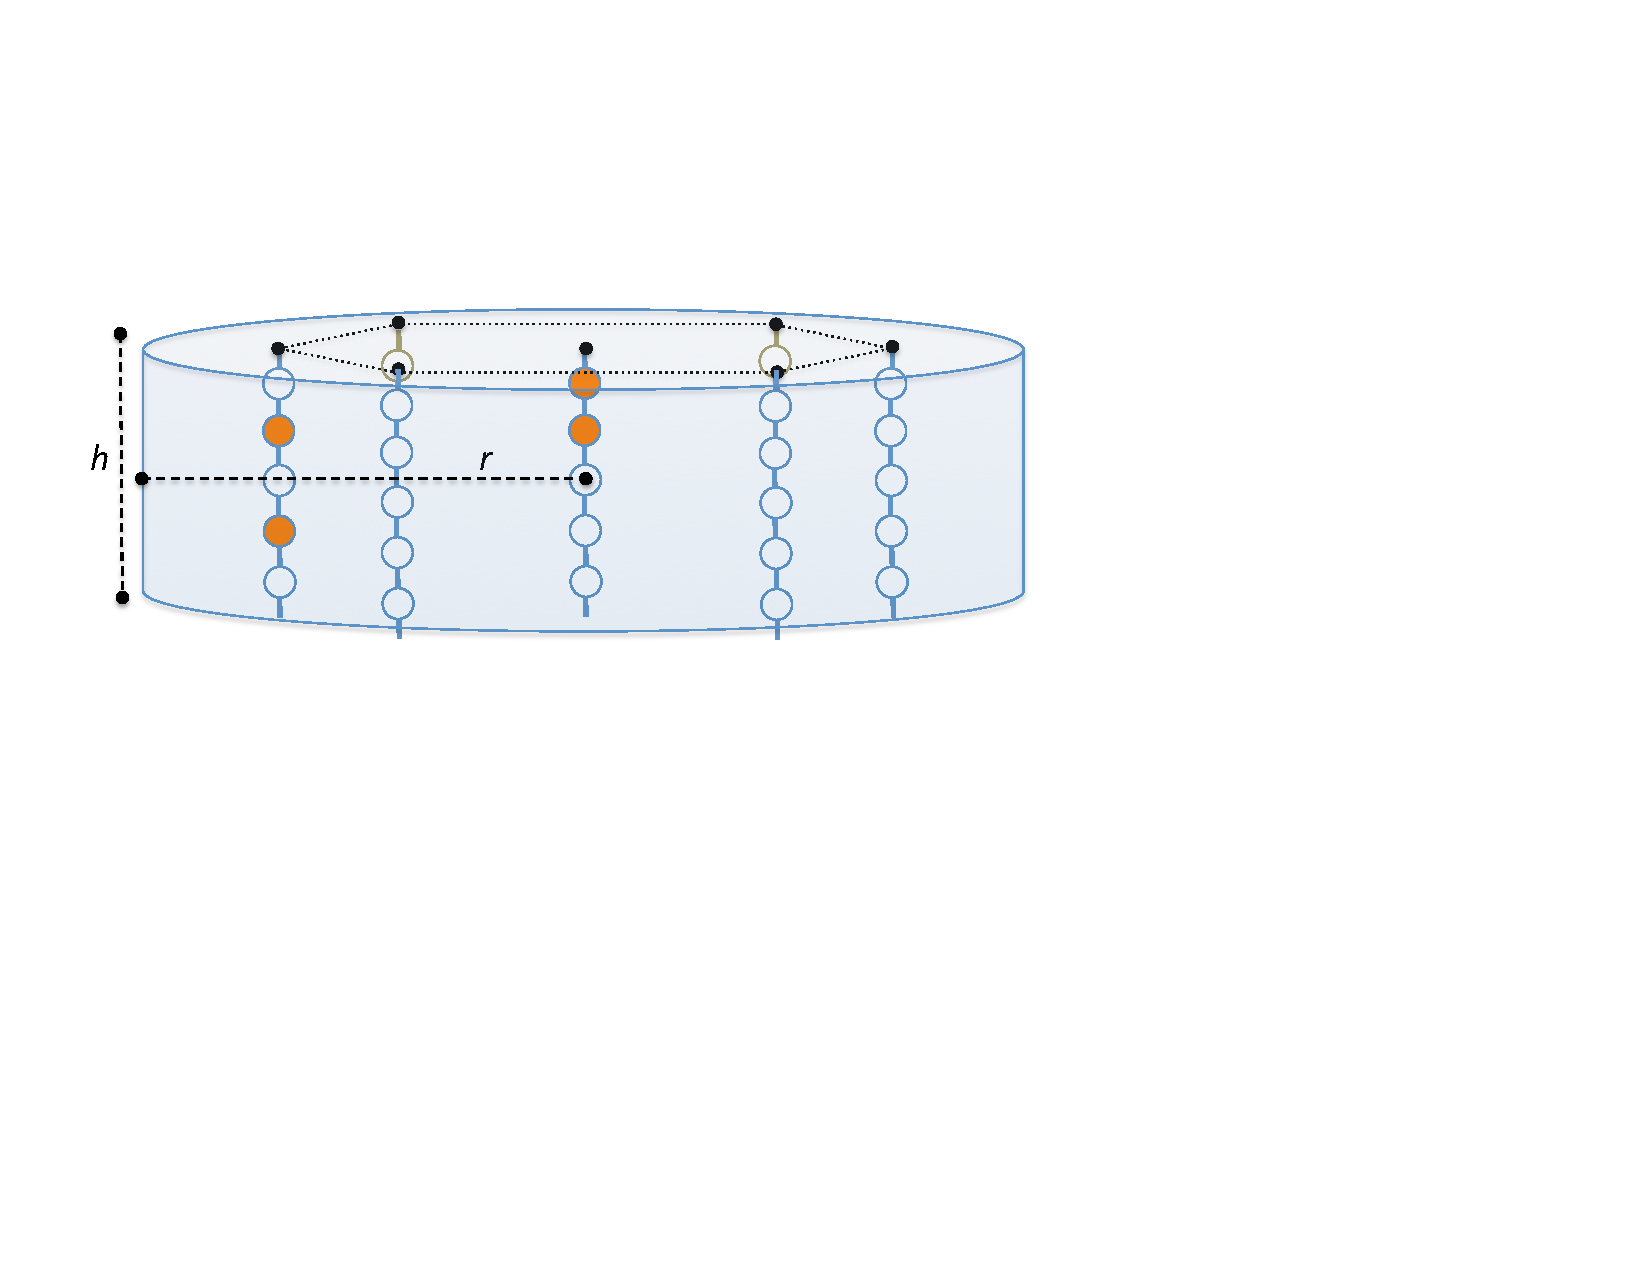
\includegraphics[scale=0.45]{graphics/online/trigger/trig_cylinder}
    \label{fig:trig_cylinder}
  }
  \quad
  \subfloat[Schematic representation of the string trigger.]{
    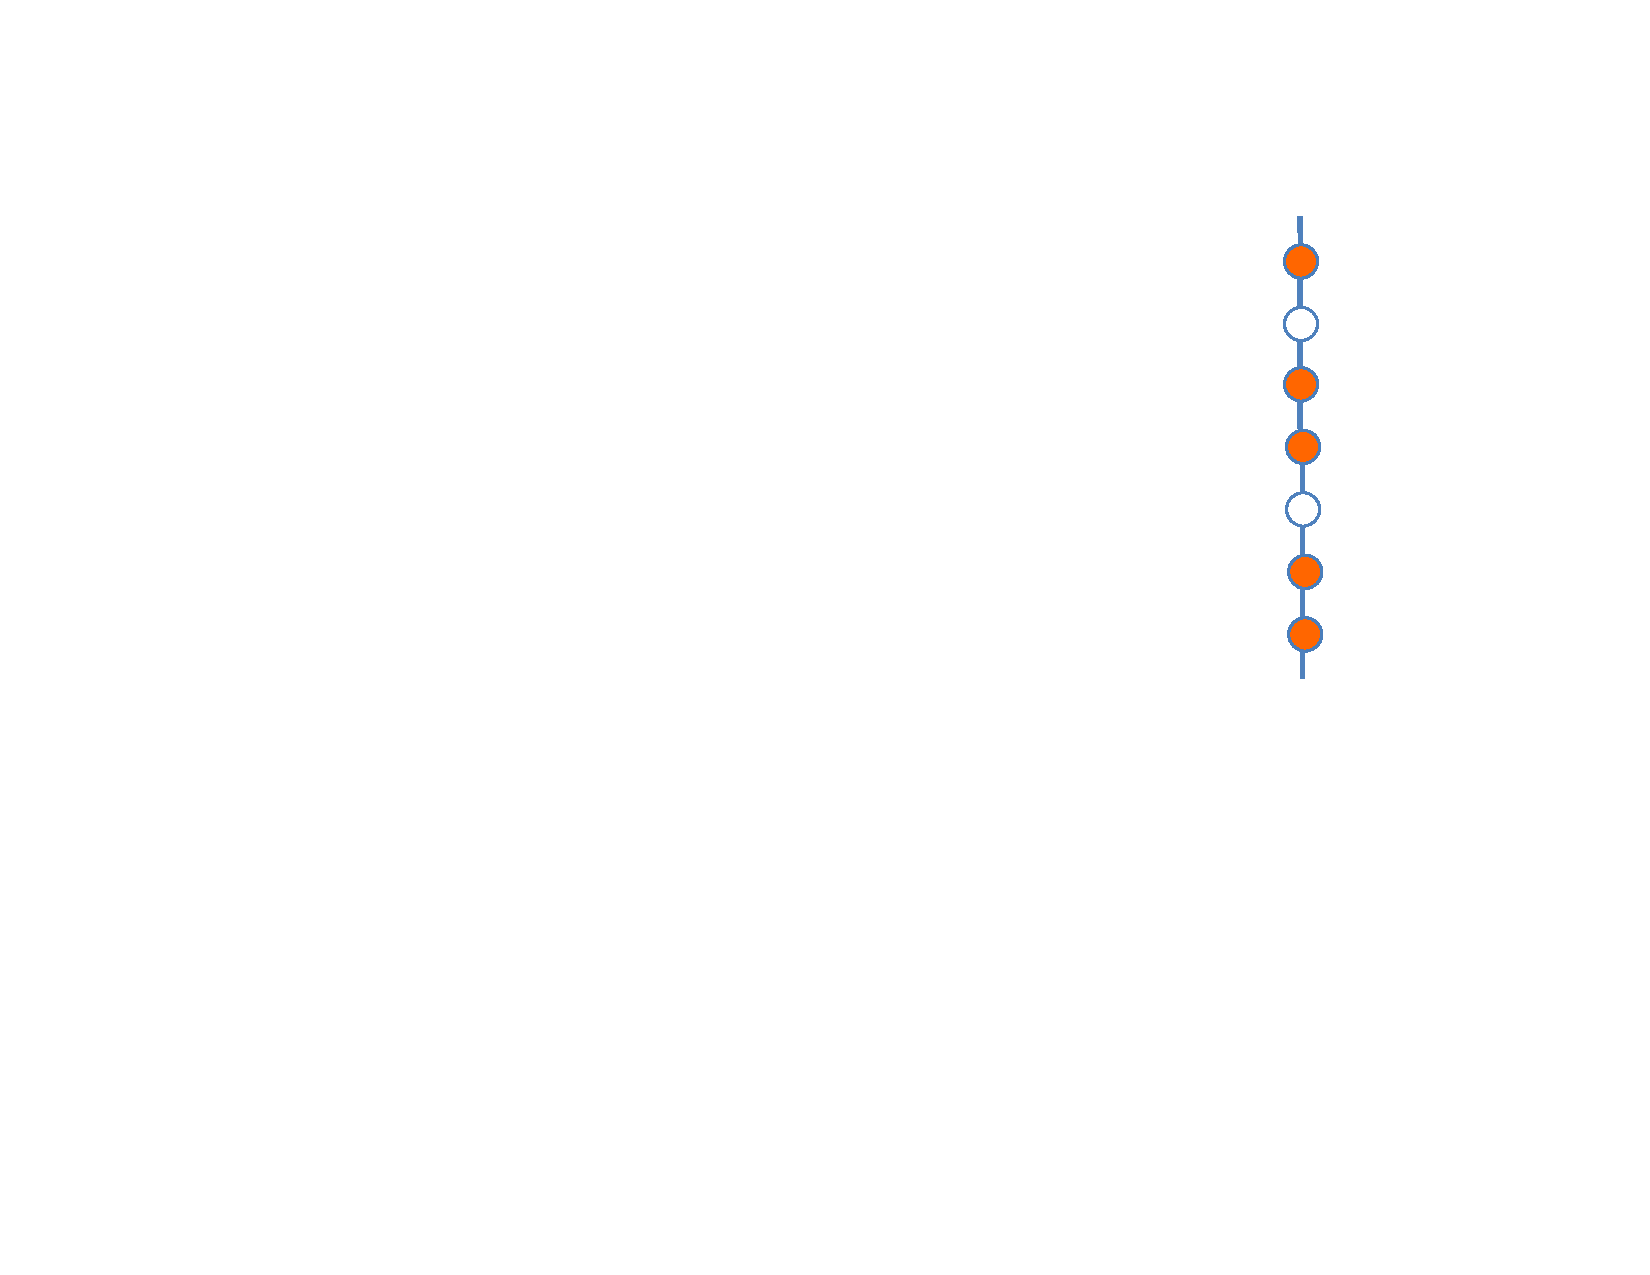
\includegraphics[scale=0.5]{graphics/online/trigger/trig_string}
    \label{fig:trig_string}
  }
  \caption{IceCube triggers using spatial coincidences.  Shaded circles represent hit DOMs.}
\end{figure}


\paragraph{Slow Particle Trigger}

IceCube has the potential to detect hypothetical subrelativistic heavy
particles such as magnetic monopoles, via catalyzed nucleon decays along
the particle trajectory \cite{IC3:monopole}.  However, because these
particles travel at velocities $v \sim 0.001c - 0.01c$, the
time windows used in the standard triggers are too short.  Therefore, a
dedicated \emph{slow particle (SLOP) trigger} has been developed to
search for slow track-like particle signatures.

The SLOP trigger operates in several stages.  HLC hits, which by
design come in at least pairs along a string, are cleaned by removing pairs
that are too close in time ($\Delta t < T_{\mathrm{prox}}$), removing
many muon hits.  Next, 3-tuples of HLC pairs within a time window
$T_{\mathrm{max}}$ are formed.  The geometry of each
3-tuple formed must satisfy track-like conditions: the obtuse inner angle
of the triangle formed must be larger than $\alpha_{\mathrm{min}}$, and the
``velocities'' along the triangle sides must be consistent.  Specifically,
the normalized velocity difference, defined as

\begin{equation}
  v_{\mathrm{rel}} =
  3(v^{-1}_{12} - v^{-1}_{23})/(v^{-1}_{12} + v^{-1}_{23} +
  v^{-1}_{13})
\end{equation}

\noindent where $\ v_{ij} = \Delta x_{ij}/\Delta t_{ij}$, must be less than
or equal to a pre-definined maximum value
$v_{\mathrm{rel}}^{\mathrm{max}}$.  Figure \ref{fig:slop} 
shows the geometry parameters of the 3-tuple.  Finally, the number of track-like
3-tuples must be greater than or equal to $N_{\mathrm{tuple}}$.  

\begin{figure}[!h]
 \centering
 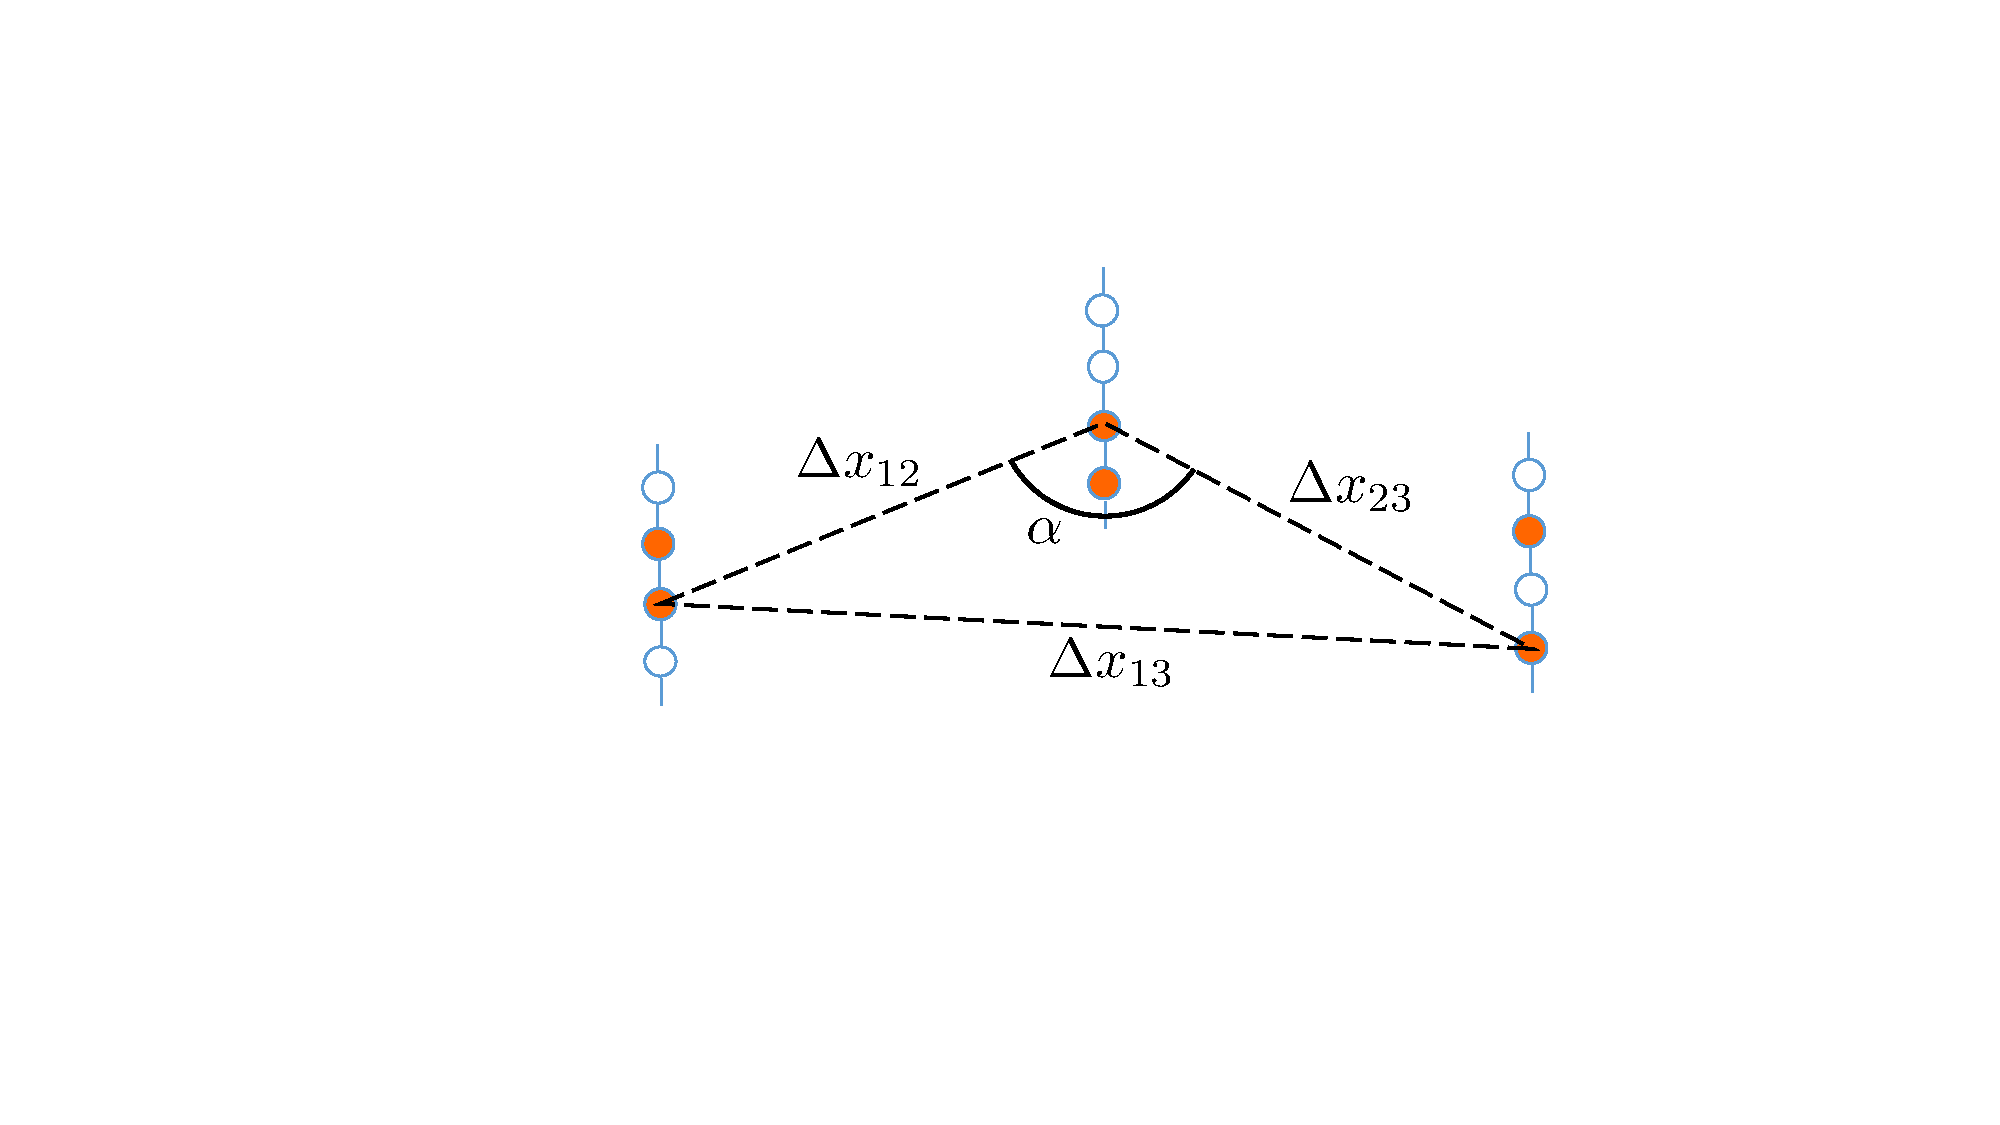
\includegraphics[width=0.8\textwidth]{graphics/online/trigger/slop.pdf}
 \caption{Geometry of a SLOP trigger HLC pair 3-tuple.}
 \label{fig:slop}
\end{figure}

\paragraph{Other Triggers}

Other special-purpose triggers exist to collect minimum bias data of
various sorts.  The \emph{fixed-rate trigger (FRT)} triggers at a given
rate and reads out 10 ms of data from the full detector.  This is especially useful
for studies of DOM noise.

FIX ME: minbias and calibration triggers

\begin{table}
  \centering
  \footnotesize
\begin{tabular}{lrrrrr}
  \hline
  Trigger & DOM set & $N$ HLC hits & Window ($\mu$s) & Topology & Rate (Hz) \\
  \hline
  SMT & in-ice & 8 & 5 & --- & 2100\\
  SMT & DeepCore & 3 & 2.5 & --- & 250\\
  SMT & IceTop & 6 & 5 & --- & 25\\
  Volume & in-ice & 4 & 1 & cylinder (r=175m, h=75m) & 3700\\
  String & in-ice & 5 & 1.5 & 7 adjacent vertical DOMs & 2200\\
  SLOP & in-ice & $N_{\mathrm{tuple}} = 5$ & $T_{\mathrm{prox}} = 2.5,
  T_{\mathrm{max}} = 500$ & $\alpha_{\mathrm{min}} =
  140^\circ,\ v_{\mathrm{rel}}^{\mathrm{max}} = 0.5$ & 12\\
  FRT & all & --- & --- & --- & 0.003\\
\hline
\end{tabular}
\caption{IceCube trigger parameters (as of May 2013) and typical trigger rates of
  each algorithm.  Most rates vary seasonally with the atmopheric muon flux.} 
\label{tab:triggers}
\end{table}

\paragraph{Trigger and Readout Window Merging}

Bright or long events will satisfy more than one of the trigger conditions,
sometimes multiple times (see Fig.~\ref{fig:trigger_example}).  In order to
avoid overlapping events, possibly containing the same DOM hits, the
triggers and their associated readout windows are merged, while retaining
information about the separate 
triggers.  The merged trigger is referred to as the \emph{global trigger}.  

Each trigger has defined readout windows around the trigger window;
all hits (including those without LC conditions) from the full detector,
including those DOM sets not involved in the trigger, are built into
events.  For the DOM set involved in the trigger, the readout 
windows are appended to the trigger window; for other DOM sets, the readout
windows are centered around the trigger start time.  The union of
overlapping readout windows defines an event; an example is shown in
Fig.~\ref{fig:trigger_readout}.  Long events (SLOP, FRT) typically contain several
independent ``physics'' events; these typically have to be re-split for
reconstruction and analysis.

\begin{figure}[ht]
  \centering
  \subfloat[Sample bright event satisfying multiple triggers.  The vertical ticks
    indicate the time of DOM hits (including SLC hits).  Trigger windows are
    illustrated with solid horizontal lines, readout windows by dashed lines.]{
    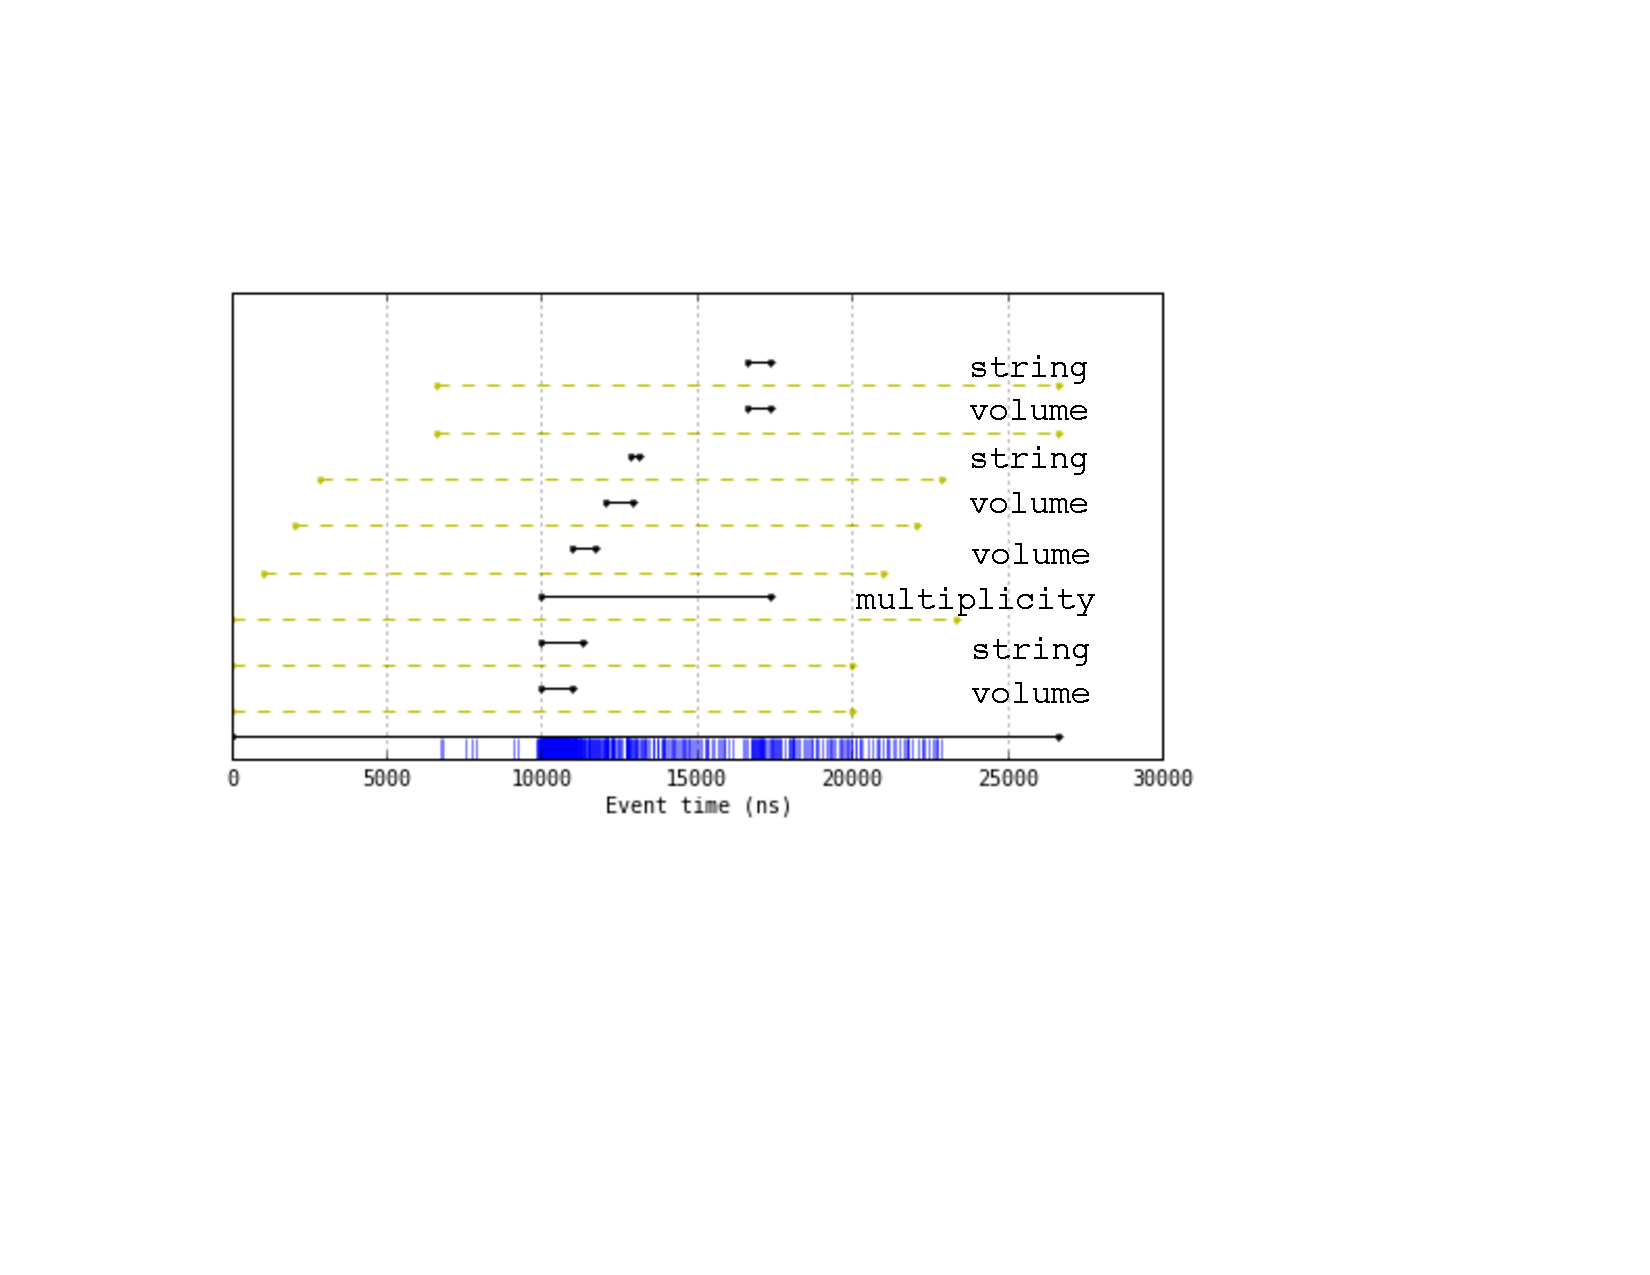
\includegraphics[scale=0.5]{graphics/online/trigger/trigger_example}
    \label{fig:trigger_example}
  }
  \quad
  \subfloat[In-ice and IceTop readout windows for a long event (SLOP trigger).]{
    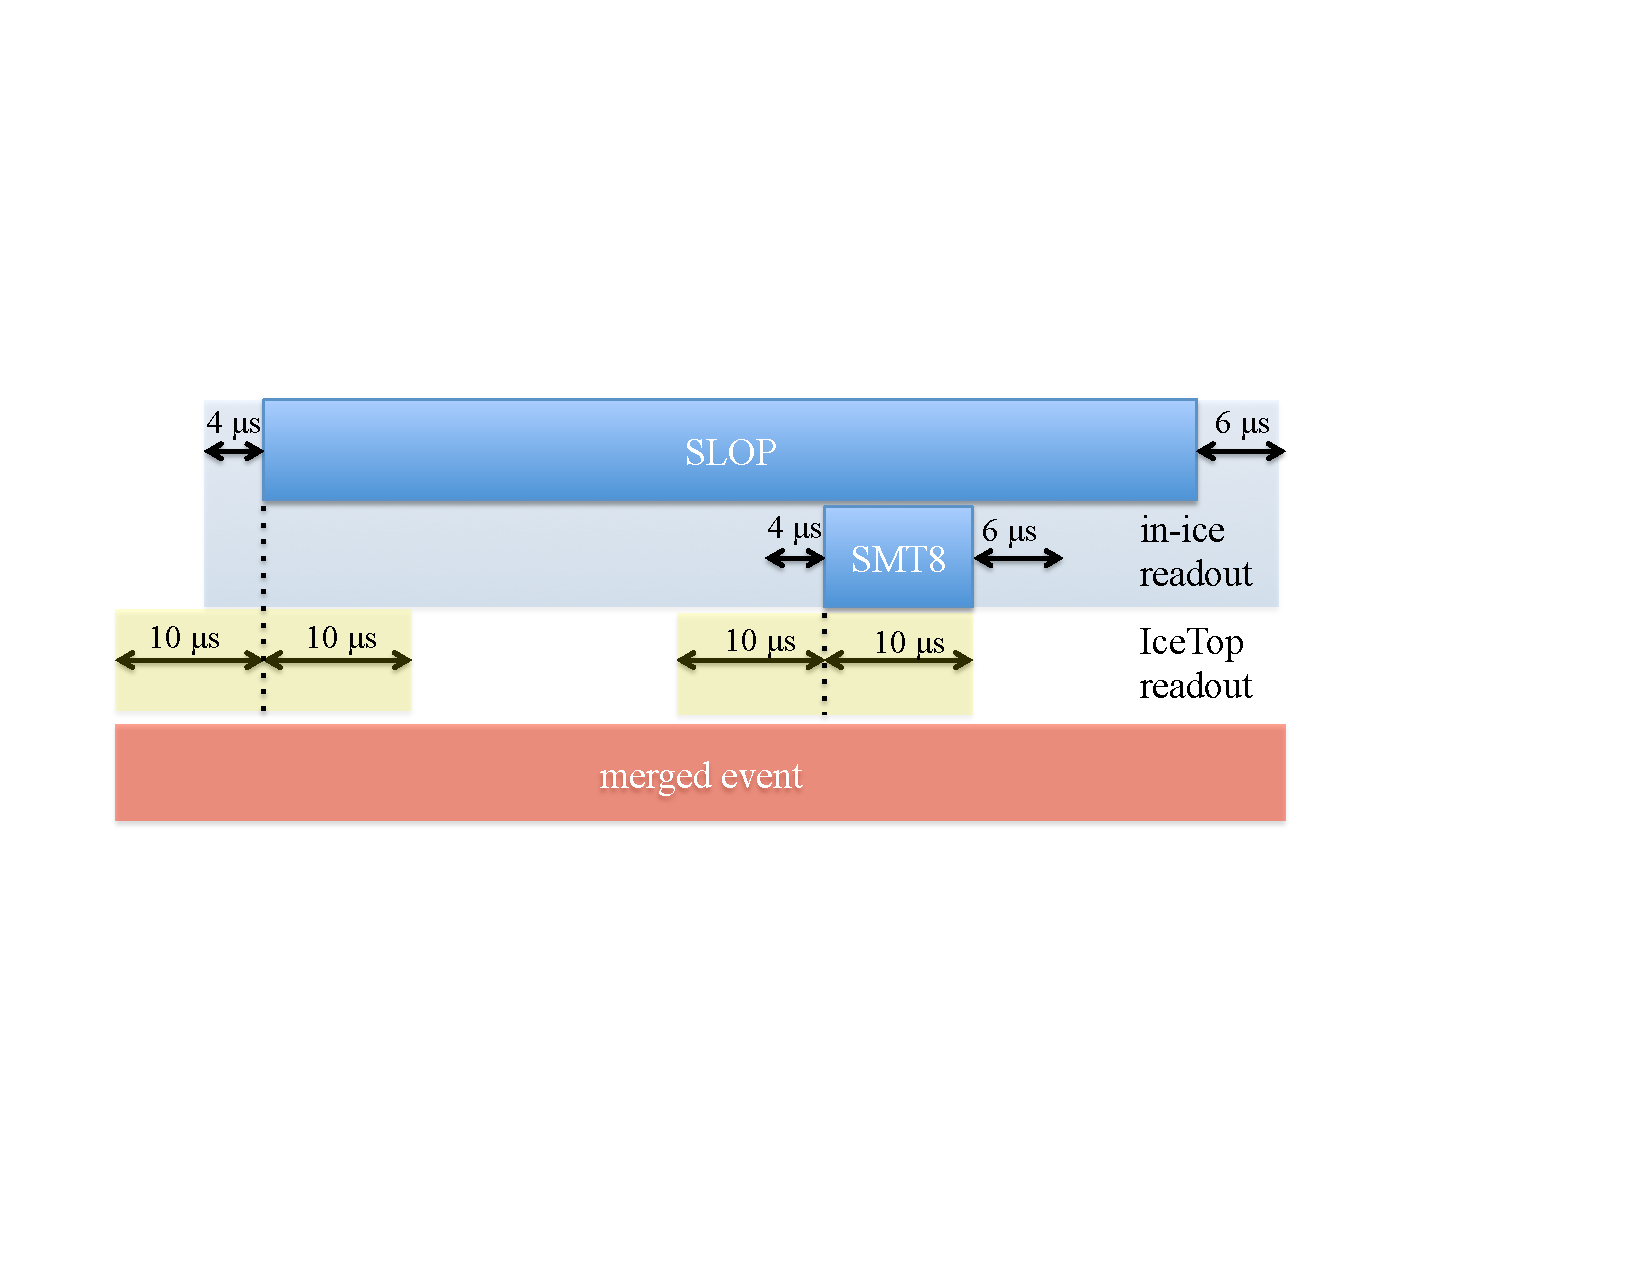
\includegraphics[scale=0.5]{graphics/online/trigger/trigger_readout}
    \label{fig:trigger_readout}
  }
  \caption{IceCube trigger and readout window merging.}
\end{figure}

%General description of trigger architecture.  Separation of trigger window
%and readout window.  How trigger windows depend on geometry.  Thorough
%description of all different trigger algorithms. Trigger and readout window
%merging.

\subsubsection{\label{sect:online:evbuilder}Event Building}

%Readout requests to StringHub components
The Event Builder receives requests from the Global Trigger, extracts
the individual readout windows, and sends them to the appropriate subset of the
hubs.  The hubs each send back a list of all hits within the window.  When all
hubs have returned a list of hits, extraneous data is removed from the trigger
and hit payloads and bundled into an event payload.

%Spooling to disk and interface to PnF.
Events are written to a temporary file.  When the temporary
file reaches a configurable size, it is renamed to a standard unique name
%(made up of a ``physics\_'' prefix, the run number, a sequentially increasing
%file number, and the starting and ending times contained within the file).
When the PnF system sees a new file, it accepts it for
processing (and filtering).

%\subsubsection{The Secondary Streams (SN/Moni/TCAL)}
%Is this necessary or can we just mention these in the StringHub section?

\subsubsection{Configuration}

Configuration of the DAQ is managed by two sets of files; a cluster
configuration file and a hierarchical tree of run configuration files.

The cluster configuration file contains system-level settings used to launch
the DAQ, such as component hosts, startup paths, command-line options, etc.
Components
(other than StringHub) can easily be moved to different hosts for
troubleshooting, load balancing, maintenance, etc.

Run configuration files list the trigger and DOM configuration files to be
used for taking data.

The trigger configuration file specifies configuration parameters for all
trigger components (in-ice, icetop, and global) used in a run.  These include
the list of algorithms run by each trigger component, along with readout window
sizes and any other variable parameters (frequency, threshold, etc.)

DOM configuration files (one per hub) list of all DOMs which contribute to the
run.  All configuration parameters for each DOM are specified.

%Modification of config files
Run configuration files (including trigger and DOM files) are frozen once
they've been used for data taking so the settings associated with each run can
be determined.  Modifications to any file in the tree must be made by copying
the settings to file with a new name.
%The cluster configuration file may be modified but a note should be sent to the
%``logbook'' email list.  Run configuration files are treated as static once
%they've been used for data taking.  If a configuration file needs to be
%altered, the modified file is given a new name (often with an incremented
%``-V\#\#\#'' suffix indicating the version number) to ensure that the exact
%detector configuration is always discoverable.

\subsubsection{Distributed Network Control}

%CnC server description.
%The central coordination point for the DAQ is a ``command-and-control'' daemon
%named CnCServer.  It manages and monitors components, and acts as the main
%external interface for the DAQ.

The DAQ components are managed by a single ``command-and-control'' daemon
which manages and monitors components, and acts as the main
external interface for the DAQ.

It uses a standard component interface to query and
control the components, and a separate interface for components to expose
internal data used for monitoring the health of the detector and tracking
down bugs and/or performance problems.

%CnCServer starts out knowing nothing about the detector components.  During the
%DAQ's launch phase, components are given the host and port used by CnCServer.
%When components start up, each one sends CnCServer its name, host/port pairs,
%and the types of inputs and outputs it expects, and CnCServer adds them to its
%internal list.

%To start a run, CnCServer is given the name of the run configuration.  That
%run configuration may include all components or only a subset.  Using
%that file, CnCServer builds a list of components required for the run.
%Each of the included components is told to connect to their downstream
%neighbor, then to use the run configuration to initialize as appropriate
%(configure DOM hardware, initialize trigger algorithms, etc.).
%Once all components are successfully
%configured CnCServer instructs them to start, working its way from the Event
%Builder back to the String Hubs.

%When a run is in progress, CnCServer regularly checks that components are still
%active and that data is flowing between components.  If it detects a problem,
%it stops the run and relaunches all the components.  CnCServer also
%periodically collects all components' monitoring data and writes it to
%monitoring files which can be used for post-mortem diagnosis of detector
%failures.

\subsection{Online Filtering}
\textsl{(Erik B.; 3-4 pages)}
\subsubsection{Overview}

The online processing and filtering system is charged with the immediate handling of all triggered events collected by the data
acquisition system and reducing the data volume to a level that can be
accommodated in our satellite bandwidth allocations ($\sim$100 GB/day).
This treatment includes application of calibration constants, application of event characterization and selections,  
extracting data quality monitoring information, generation of realtime alerts for events of astrophysical interest
and creation of data files and metadata information for long term archiving.  The online processing and filtering system
is a custom software suite that utilizes a computer cluster of $\sim$20 standard servers located in SPS computing cluster.
The online processing and filtering system has been in operation since the
start of operation of the 22 string configuration of IceCube in 2007.

In IceCube, each triggered event consists of a collection of digitized waveforms recorded by the digital optical modules (ref daq-dom paper).
To be useful for physics, each of these waveforms requires application of calibration constants that allow the waveform units
to be converted from the raw units (ADC counts per sample bin) to more physical units (mV measured in each fixed time, 3.3 ns bin).  These
calibration constants are independently measured (see domcal section) and stored in an online database for use by
the online processing and filtering system.  Next, each DOM's waveform is deconvolved using the known DOM response
to photons to extract the light arrival time and amplitude information~\cite{IC3:ereco}.  
This series of time and amplitude light arrival information
for each DOM is the base for event reconstruction and characterization.  The online processing and filtering system encodes
this information for each DOM in a compact data format known as the SuperDST, and occupies 9\%  of the file size
of the full waveform information.  This encoding does introduce a small level of discretization error to the
data in SuperDST format, measured to be $1.1ns$ in time and $0.04pe$ in charge, and smaller than the calibration
uncertainties on these values.  Any DOM readout whose SuperDST information is found not to be a good representation of the
original waveform, or sees very high amounts of light also have the full waveform readout saved as an addition to the SuperDST record.

% JVS internal study on discretization:  
% https://events.icecube.wisc.edu/getFile.py/access?contribId=140&sessionId=4&resId=0&materialId=slides&confId=33

Each event is then characterized with a series of event reconstruction algorithms that attempt to match
the observed patterns of recorded light in the SuperDST with known patterns of light
from track and showering event hypotheses (ref reco papers?  e-reco paper?).  These characterizations (location, direction, and energy) and their
overall goodness-of-fit produced by these reconstructions are used to select interesting
events by a filter selection.  The filter criteria are set by the IceCube collaboration for each season
and are tuned to select events of interest to specific analyses.  Each season there are
about 2 dozen unique filter selections in operation.  Some of these filters trigger are
designed to search for neutrino events of wide astrophysical interest to the scientific community and trigger
alerts that are distributed to followup observatories worldwide. (ref SN-OFU paper, others?)

The online processing and filtering system also extracts and aggregates data quality and monitoring information
from the data as is it processed.  This information includes stability and quality information from the
DOM waveform and calibration process, rates of DOM readouts, and rates and stability
information for all detector triggers and filters.  This information is aggregated for each data segment and
reported to the IceCube Live monitoring system.

Finally the online processing and filtering system writes several data files that make up the long-term data archive of the IceCube
experiment.  These include:
\begin{itemize}
\item \emph {Filtered data files} These files contain only events selected by the online filter selections.  These events
generally only include the SuperDST version of the DOM information and results from the online event reconstructions.  These
files are queued for transmission to the IceCube data warehouse by the data handling system using the TDRS satellites.
\item \emph {SuperDST data files} These files contain the SuperDST version of DOM readout information for all triggered events as well as summary
information from the online filtering process.  This file set is intended as the long-term archive version of IceCube data.
\item \emph {Raw data files}  These files contain all uncalibrated waveforms from all DOMs for every event.  This large data
set is saved until final data quality assurance on the SuperDST sample can be completed.
\end{itemize}

During normal operations, the data acquisition system produces a raw data output of $\sim$1 TB of raw data per day, which result in
a raw data file archive of the same size.  The SuperDST  and filtered data archive, after data compression, are $\sim$170 GB/day and $\sim$90 GB/day,
respectively.  (TODO: verify these numbers.)
\subsubsection{System Design}

The online processing and filtering system uses a modular design, where each component
is responsible for a portion of data processing built around a central master server node and a
scalable number of processing client nodes.  The central master server focuses on
data distribution and aggregation tasks (requesting data blocks from the DAQ, collating event SuperDST, reconstruction, filter,
and monitoring information and writing data files), while the client process focus on the per-event
processing tasks (event calibration, reconstruction, analysis, and filtering).  

The system is built upon the IceCube analysis software framework, IceTray (ref?), allowing standard IceCube algorithms to
be used in the online processing and filtering system without modifications.  Additionally, the system uses the 
Common Object Request Broker Architecture (CORBA) system as means for controlling, supervising and interconnecting
the modular portions of the system.  Specialized classes are used to provide CORBA interconnections
within the IceTray system, allowing file-like interfaces that let data to stream from one component to another
using native IceTray formats.  Use of a CORBA name server and a dynamic architecture allow for the
addition and remove of filtering clients as needed to meet the processing load from annual filtering
changes and overall rate variations from seasonal variations in the detector trigger rate or moving system components within the SPS
computer system as needed.

\subsubsection{Components}
The flow of triggered event data in the online processing and filtering system is shown in Figure~\ref{fig:online_pnf_internals}
highlighting the flow of data from the DAQ system, though the master server and clients, to files on disk and
online alerts.  Several standard components in the online processing and filtering system include:
\begin{itemize}
\item \emph {DAQ Dispatch} is a process to pickup event data from the data acquisition system data cache and forward to
the PFServer components.
\item \emph {Central Server} are central data flow managers within the  online processing and filtering system.  These servers 
receive data from the I3DAQDispatch event source, distribute events to and record results returning from the PFClient farm,
and send events to file, monitoring and alert writing components.  Typically there are 4 servers used
in operation.
\item \emph {Filter Clients} is the core calibration, reconstruction and filtering process that is applied to each triggered event.  
In normal operation, up to 500 of these clients operate in parallel to filter events in real time.
\item \emph {DB Dispatch} is a DB caching system to prevent the ~400 PFClient processes from overwhelming the 
DB system when requesting calibration information.  This system aggregates DB requests, makes a single
database query and shares the results with all PFClients.
\item \emph {File Writers} are responsible for creation of files and meta-data for the IceCube data archive.  These
files are written in standard IceTray file format.  There is one writer component for each file type created.
\item \emph {Online Writer} is responsible for extracting event reconstruction and filter information from the data for events of astrophysical interest 
and sending this information out  in real time via the IceCube Live alert system.
\item \emph {Monitoring Writer} is responsible for aggregating per-event monitoring information, creating histograms
and forwarding them to the IceCube Live monitoring system.  
\item \emph {Filtered Data Dispatch} and FollowUp clients are responsible for looking for bursts of neutrino events on timescales from 100 seconds up to
3 weeks in duration. This post-filtering search of the data has all filter-selected events available, enabling event to event correlations to discovered.  Any 
significant burst of neutrinos found generates alerts sent to partner observatories worldwide.
\end{itemize}

\begin{figure}[!h]
 \centering
 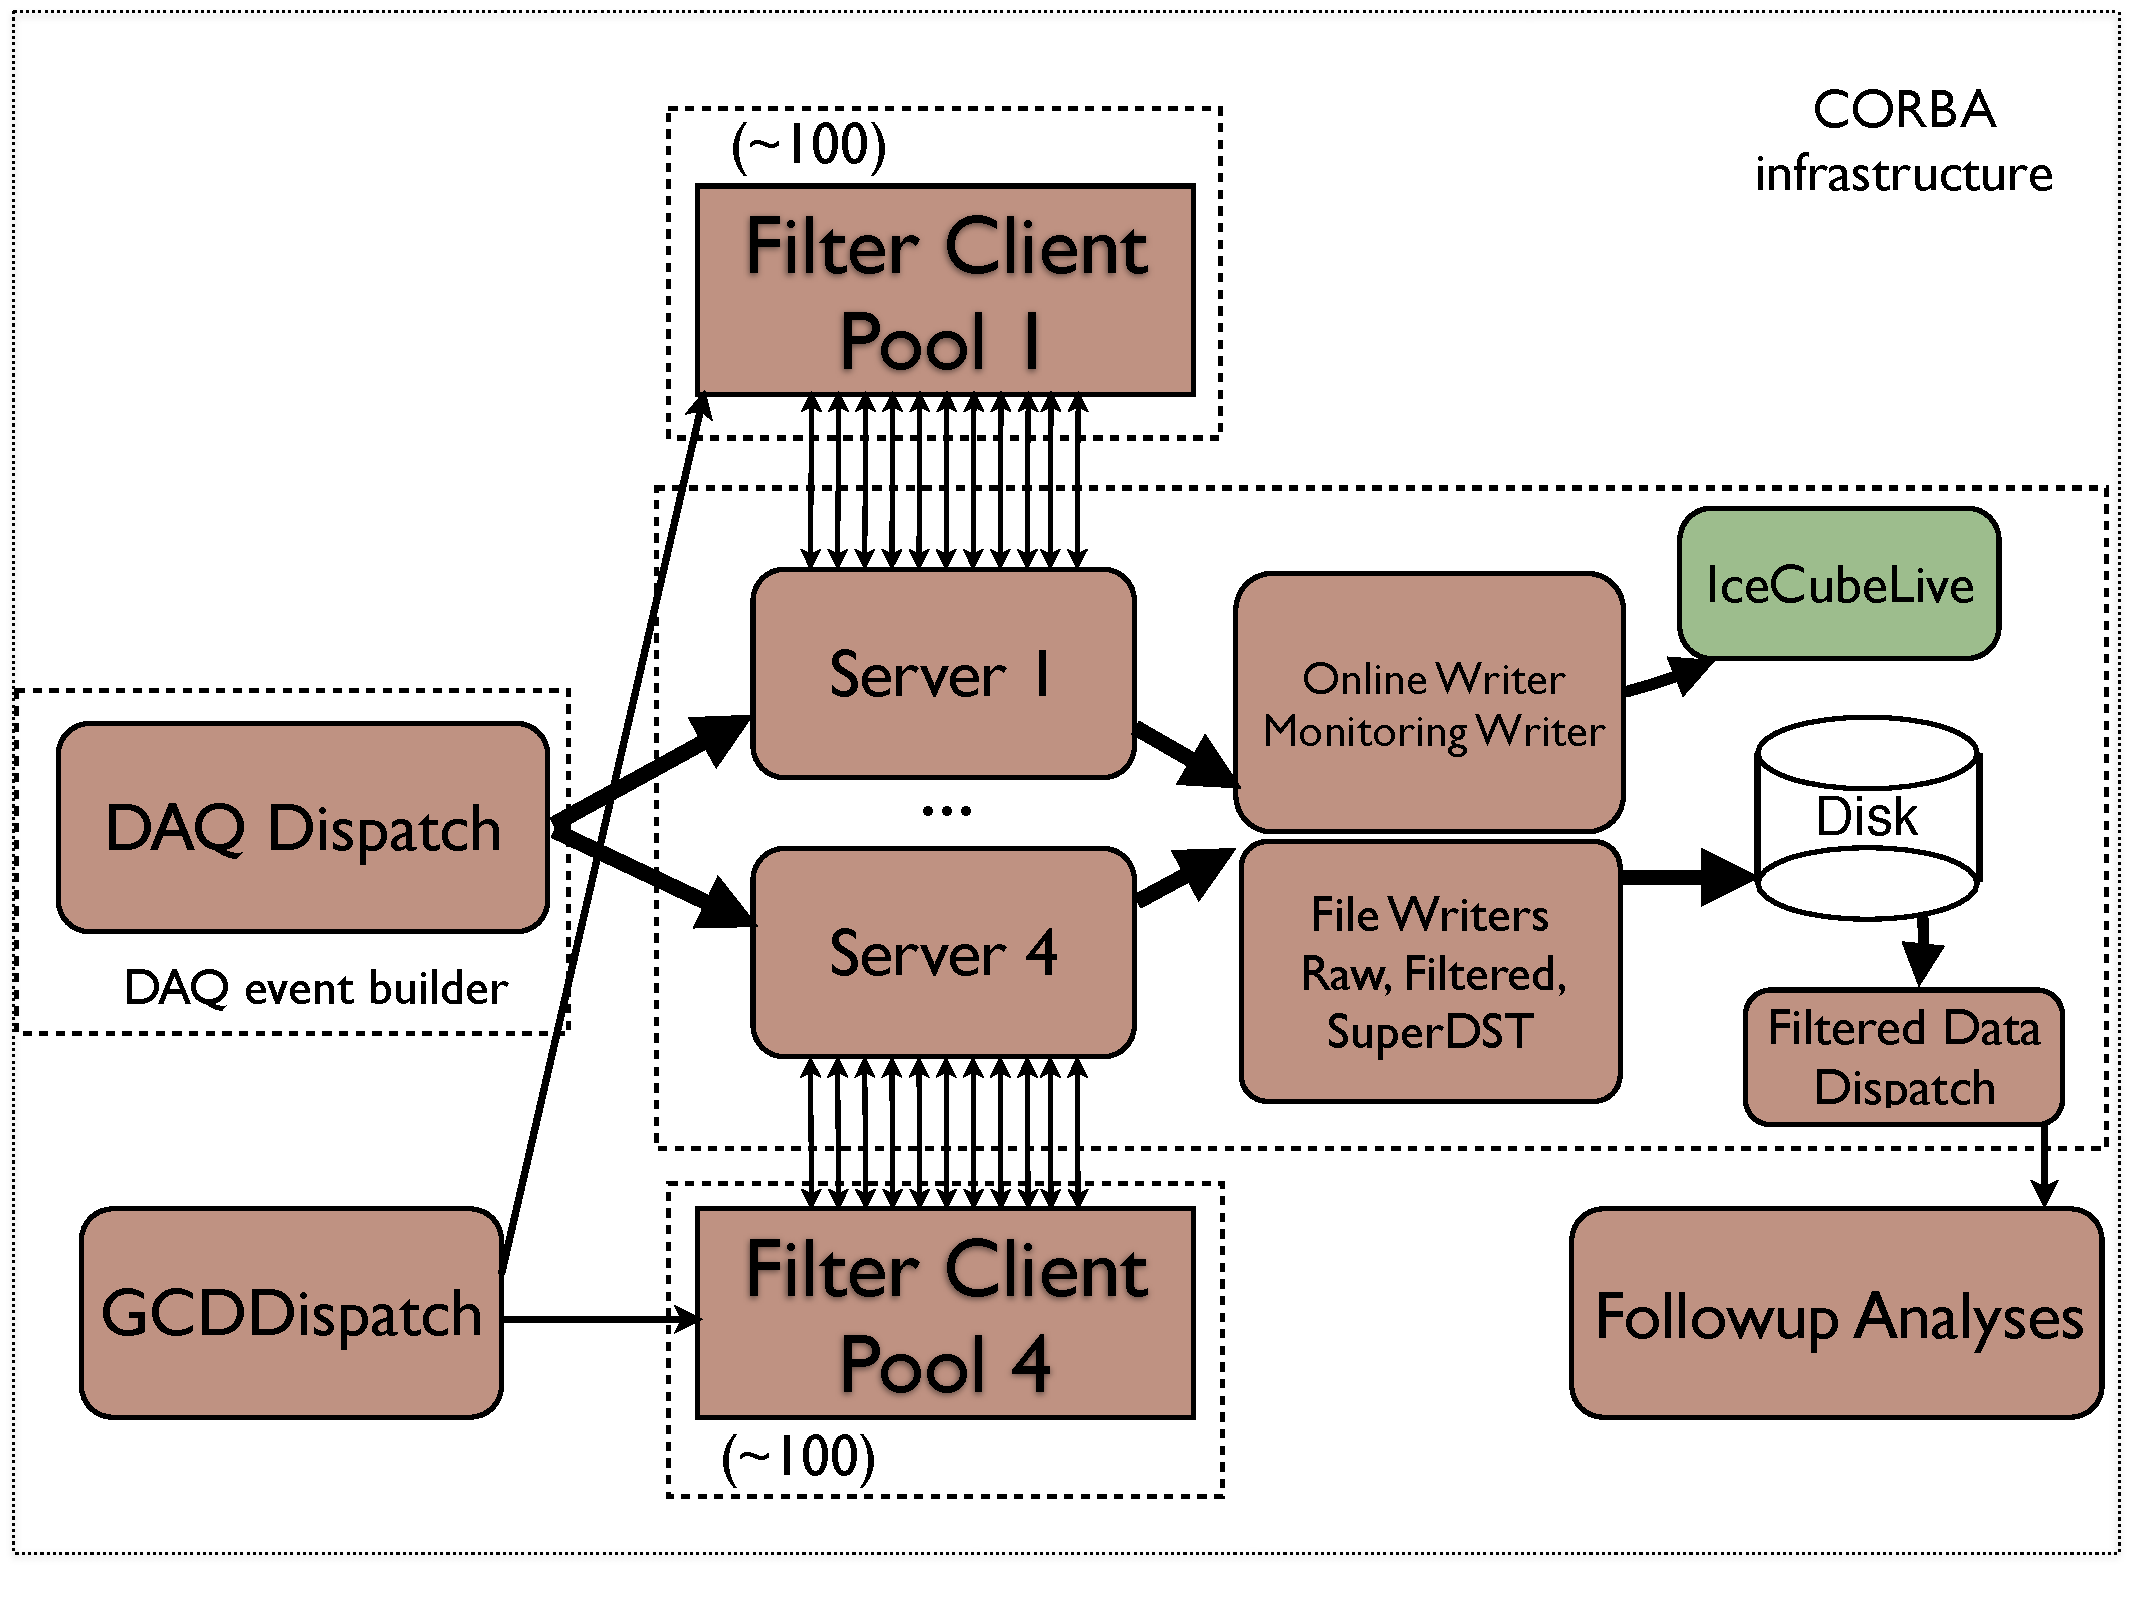
\includegraphics[width=0.8\textwidth]{graphics/online/pnf/PnF_Internals.pdf}
 \caption{Internal components of the Online Processing and Filtering System.  Arrows highlight the flow of data within the system.}
 \label{fig:online_pnf_internals}
\end{figure}

\subsubsection{Performance}
The online processing and filtering system is designed to filter triggered events as quickly as possible after collection by
the data acquisition system.   A key metric is processing system latency, defined as the duration of time between the data acquisition trigger
and the completion of event processing and filtering.  A typical latency history for the system is shown in Figure~\ref{fig:online_pnf_latency}, showing
typical system latencies of $\sim$20 seconds.

\begin{figure}[!h]
 \centering
 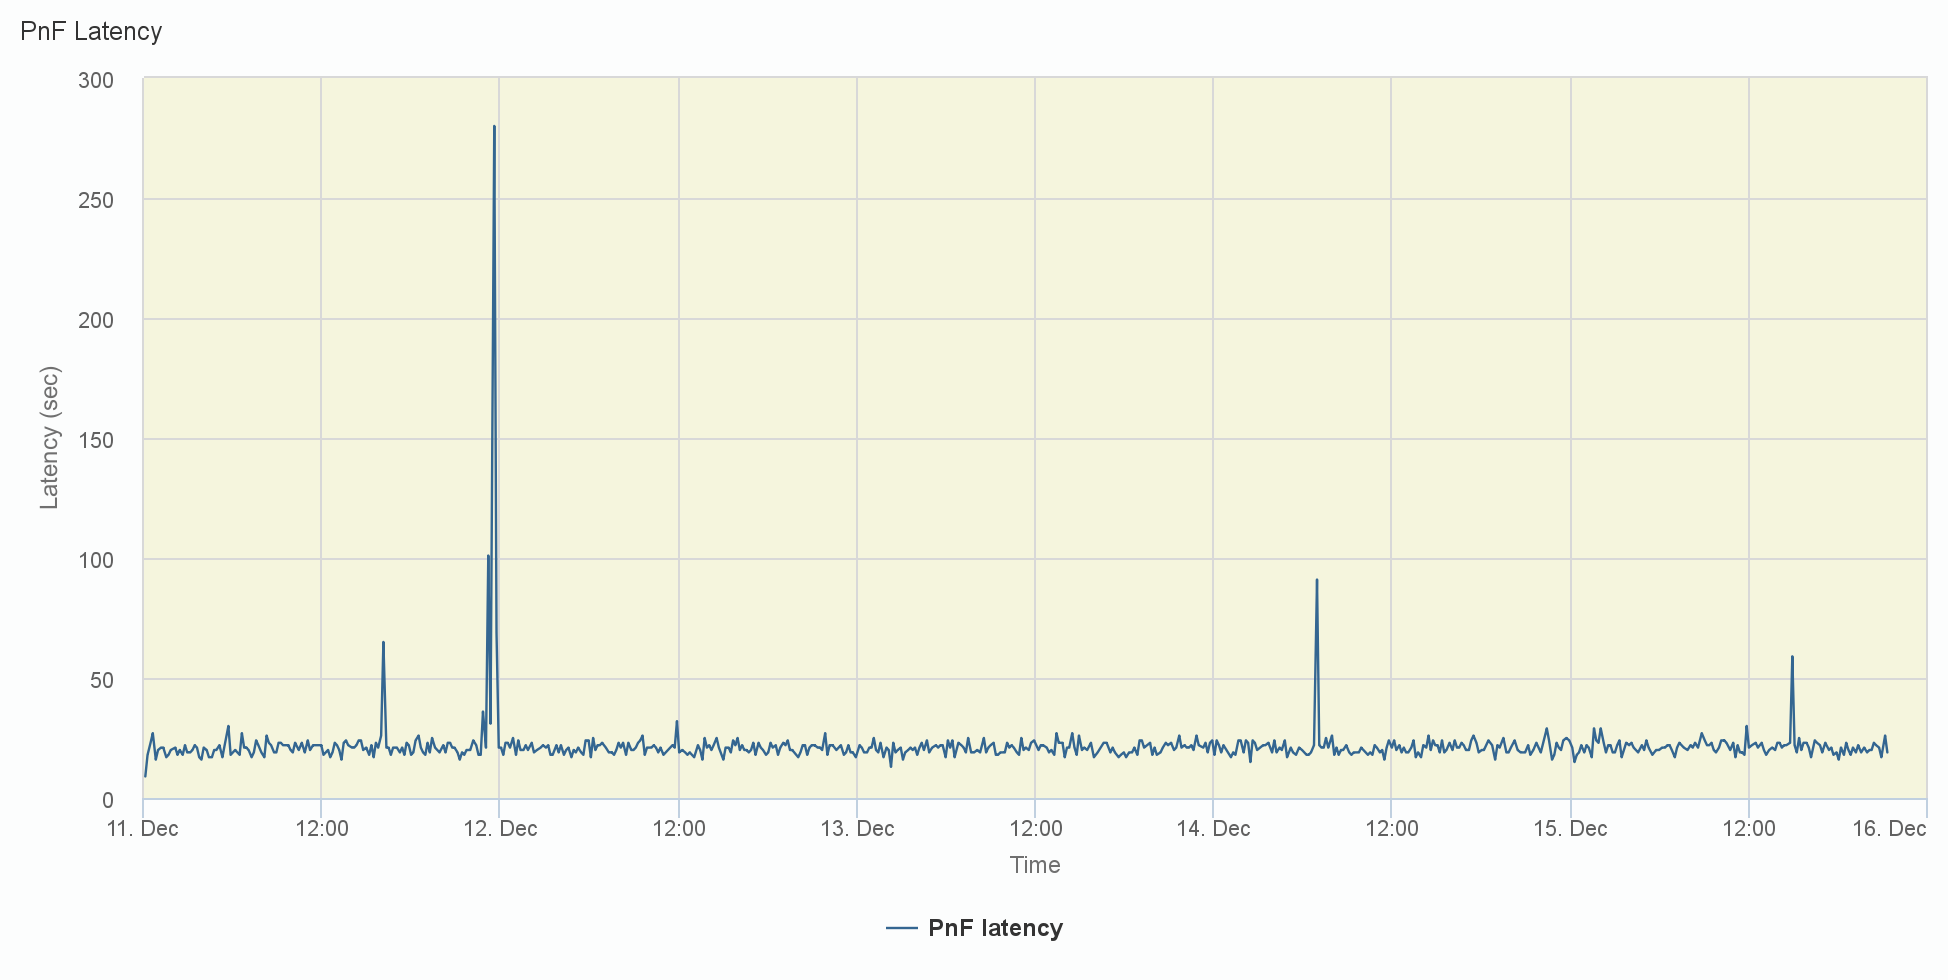
\includegraphics[width=0.8\textwidth]{graphics/online/pnf/pnf_latency.png}
 \caption{Typical Online Processing and Filtering System latency for a several day period.  The latency defined as the time between DAQ event time and time when the
 online filtering processing is complete.  The spikes in latency correspond to DAQ run transitions.}
 \label{fig:online_pnf_latency}
\end{figure}

(Q: include other system performance information?  Performance bottlenecks?)

\subsection{Data Handling}
\textsl{(P. Meade; 1 page)}

\textsl{(J. Braun, background and additional description of communications modes)}

The bulk of South Pole Station data traffic is handled by geosynchronous satellite links.  Due to the unfavorable
location at the South Pole, only geosynchronous satellites with steeply inclined orbits reach far enough above the
horizon to establish a link.  For a given satellite, this link provides four to six hours of communications once per
sidereal day.  Multiple geosynchronous satellites are currently utilized by USAP, providing a $\sim$12-hour window
of connectivity with bandwidth of 1 Mbps or higher.  For the remainder of the day, Iridium satellites allow
limited voice and data connectivity and provide up to 2.4 kbit/s of bandwidth per connection.

IceCube incorporates Iridium modems into two separate systems.  The IceCube Teleport System (ITS) uses the Iridium short burst
data mode to send short messages of 1.8 kB or smaller with a typical latency of 30 seconds.  Messages may both originate or terminate
at the ITS Iridium modem at the South Pole.  Messages also contain a recipient ID indicating the intendend host to receive
the message, allowing a many-to-many communications infrastructure between systems running at the South Pole and systems
in the Northern Hemisphere.  The IceCube Messaging System (I3MS) incorporates multiple Iridium modems and uses the Iridium RUDICS
data mode, providing a 2.4 kbit/s bidirectional serial stream per modem and a minimum latency of $\sim$1.5 seconds.
I3MS runs as a daemon on both ends of the link, accepts messages via ZeroMQ, and transports those messages across the link
based on message priority and fair sharing of bandwidth among all users.  I3MS message recipients listen for messages
using ZeroMQ PUB-SUB, allowing a given message to be sent to multiple recipients.

\textsl{Generation description of system architecture.  Stream definitions, dropboxes,
and data pickup.  Archival vs. transfer to TDRSS system.  }

Data handling is provided by three servers named jade02, jade03, and jade04. The jade servers operate independently of one another and
each of them are capable of handling the nominal data volume by itself. Having three servers allows for data handling to continue seamlessly
in case of hardware failure or maintenance.

Each server runs a copy of the Java Archival and Data Exchange (JADE) software (stylized “jade”). As its name implies, the jade software
is written in the Java programming language. It is a reimplementation and expansion of earlier prototype software called South Pole Archival
and Data Exchange (SPADE), written by Cindy Mackenzie. The jade software has four primary tasks: consumption, archival, satellite transmission, and real-time
transmission.

The jade software is configured with a number of data streams, which consist of a data server, a dropbox directory, and a filename pattern.
The data stream dropbox directories are checked on a regular basis for new files. A file pairing scheme (binary and semaphore) prevents files
from being consumed before they are finished being produced. For each file, a checksum calculated on the data server is compared to a checksum
calculated on the jade server. This method ensures that the file was copied without error. After this, the original data file is removed from the data host.

After consumption, files are routed according to the configuration of their data stream. Files that are too large to send via the satellite link are archived to
a configurable number of archival media copies. The prototype SPADE software archived to LTO tapes, while the later jade software archives to large (2+ TB) hard
disk drives. All of the archival data is buffered on the jade server until the archival media is complete. In case of failure while creating the archival media,
all of the files can be immediately written to fresh archival media with a single command.

Files that are too large to send via the real-time link, but small enough to send via the satellite link are queued for satellite transmission. The jade software
attempts to bundle multiple files together into 1 GB bundle archives to allow satellite link operators to manage the daily data transmission. Very large files
(>1 GB) are split apart into multiple 1 GB bundles for the same reason. The jade software will only transfer a configurable number of bundles to the satellite
relay server. If satellite transmission is not possible, the jade software will buffer the excess bundles on the jade server, to avoid flooding the relay server
unnecessarily.


Small files (<50 KB) with high priority status information are sent via the real-time link. The real-time link is provided by the IceCube Messaging Service
(I3MS). The jade software uses JeroMQ, a pure Java implementation of the ZeroMQ (ZMQ) protocol, to connect to I3MS. In cases where the real-time link is not
available, I3MS will queue the messages to be sent when the link becomes available. All I3MS messages are also sent to jade to send via the satellite link to
ensure delivery if the real-time link should be unavailable for an extended period of time.

\subsection{IceCube-Live and Remote Monitoring}

IceCube operations are controlled and monitored centrally by IceCube-Live, a suite of high-level software implemented mostly in the Python language.
IceCube-Live consists of two major components: LiveControl, responsible for controlling data-taking operations and
collecting monitoring data, and the IceCube-Live website, responsible for processing and storing monitoring data as well as presenting this data
in webpages and plots that characterize the state of the IceCube detector.

\subsubsection{LiveControl}

LiveControl executes in the background as a daemon and accepts user input via XML-RPC.
Operators typically enter commands and check the basic detector status using a command-line interface.  LiveControl is
responsible for controlling the state of DAQ and online-processing, starting and stopping data-taking runs, and recording
the parameters of these runs.  Stardard operation is to request a run start, supplying a configuration file specifying the DOMs to include in
data taking.  LiveControl then records the run number, configuration, start time, etc. and sends a request for DAQ to
begin data taking.  After data taking commences successfully, LiveControl waits a specified amount of time, generally eight
hours, then stops the current run and automatically starts a new run using the same configuration.  This cycle continues until
stopped by a user request or a run fails.  In case of failure, LiveControl attempts to restart data taking by starting a new
run.  Occasionally a hardware failure occurs, and it is impossible to start a run with the supplied configuration because requested DOMs are
unpowered or temporarily unable to communicate with the IceCube DAQ.  In this case, LiveControl cycles through predefined partial-detector
configurations in an attempt to exclude problematic DOMs.  This results in taking data with half of the IceCube strings or fewer, but it
greatly reduces the chance of a prolonged complete outage where no IceCube data is recorded.

A secondary function of LiveControl is the collection, processing, and forwarding of monitoring data from DAQ, online-processing, and other components.
Monitoring data consists of a JSON dictionary with a well-definied format including a creation time, sender name, priority, data name, and either JSON data
or a single integer or floating-point value.  This data is forwarded to LiveControl using ZeroMQ and queued internally for processing.  A few monitoring
quantities indicate serious problems with the detector, e.g. the online-processing latency is too high.  LiveControl provides a database of checked monitoring
values indexed by service and data name and raises an alert if the value is out of the specified range or hasn't been received in a specified amount of time.
The alert usually includes an email to parties responsible for the affected subsystem and, for serious problems, triggers an automated page to winterover operators.
Several other types of monitoring data trigger a response by LiveControl.  These include alerts generated internally by subsystems, and such alerts may trigger emails
and pages from LiveControl.  All monitoring data are forwarded to the IceCube-Live website for further processing and display.

\subsubsection{IceCube-Live Website}

\begin{table}[!ht]
\begin{tabular}{|c|c|c|c|c|}
\hline
Priority & Transport System & Daily Messages & Daily Data & Typical Latency\\
\hline
1 & ITS (Iridium) & 10,000 & 1 MB & 1 minute \\
\hline
2 & I3MS (Iridium) & 150,000 & 5 MB & 1--5 minutes \\
\hline
3 & JADE (Geosynchronous) & 300,000 & 100 MB & 1 day \\
\hline
\end{tabular}
\caption{Statistics for IceCube monitoring messages}
\label{i3messages}
\end{table}

Two operational copies of the IceCube-Live website exist: one inside the IceCube network at the South Pole, and
one in the Northern Hemisphere.  Monitoring data reaches the northern website based on priority and using
both geosynchronous and Iridium data transport, summarized in table \ref{i3messages}.

Messages reaching the website are processed by the DBServer daemon and inserted into one of several database tables depending on content.
Messages also may contain directives requesting DBServer to send email, by specifying email recipients and content,
or requesting that the monitoring message be published using ZeroMQ PUB-SUB, allowing the message to be passed to an external process.  The IceCube-Live
website itself uses the Django framework and contains pages that create sophisticated views of monitoring data stored in the database.
These pages include a front page displaying active alerts and plots of event rates and processing latencies from the previous few hours, and
a page for each run that displays start time, stop time, and other essential data.  The run page contains low-level diagnostic data that
includes e.g. charge histograms, digitizer baselines, and occupancy for each DOM, and is used to diagnose problems with detector components
that occurred during the run and to determine if the run can be used in physics analysis.

Finally, the IceCube-Live website in the Northern Hemisphere transmits messages to LiveControl using ITS and I3MS.  This capability is used to retransmit
messages sent using the popular Slack chat service to the South Pole, allowing the IceCube winterover operators to chat with
experts in the Northern Hemisphere during periods with no geosynchronous satellite connectivity.  This connection also provides a limited
capability to control the detector, allowing operators in the north to e.g. remotely issue HitSpool requests.

\subsection{Operational Performance}
\textsl{(Matt K; 1 page)}

(Explanation of how design choices, system monitoring, and winterovers result in
high uptime.  Discussion of median downtime and various causes of downtime.
Possible basic failure analysis of hardware components.)

Full detector operational uptime is highly valued. Many redundancies and fail-safes have been implemented to achieve an average uptime of greater than 99\,\%. Each computing hub and server is equipped with redundant power supplies which are buffered with redundant UPSs. The detector can remain fully operational for 25 minutes in the event of a power outage. 

The Nagios monitoring infrastructure is incorporated into all IceCube subsystems and communicates with IceCube LiveControl to send out alerts, page the Winter Overs, and/or automatically initiate an alternate run configuration in the event of component failure. 

\begin{figure}[!h]
 \centering
 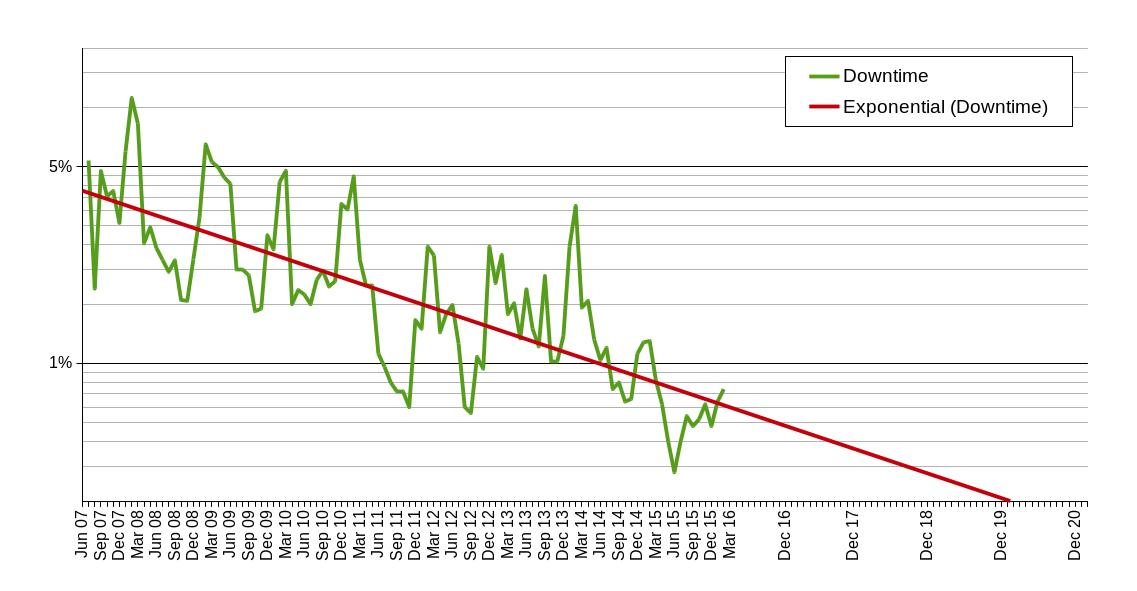
\includegraphics[width=0.8\textwidth]{graphics/uptime/downtime.jpg}
 \caption{Downtime of the IceCube detector.}
 \label{fig:downtime}
\end{figure}

\begin{figure}[!h]
 \centering
 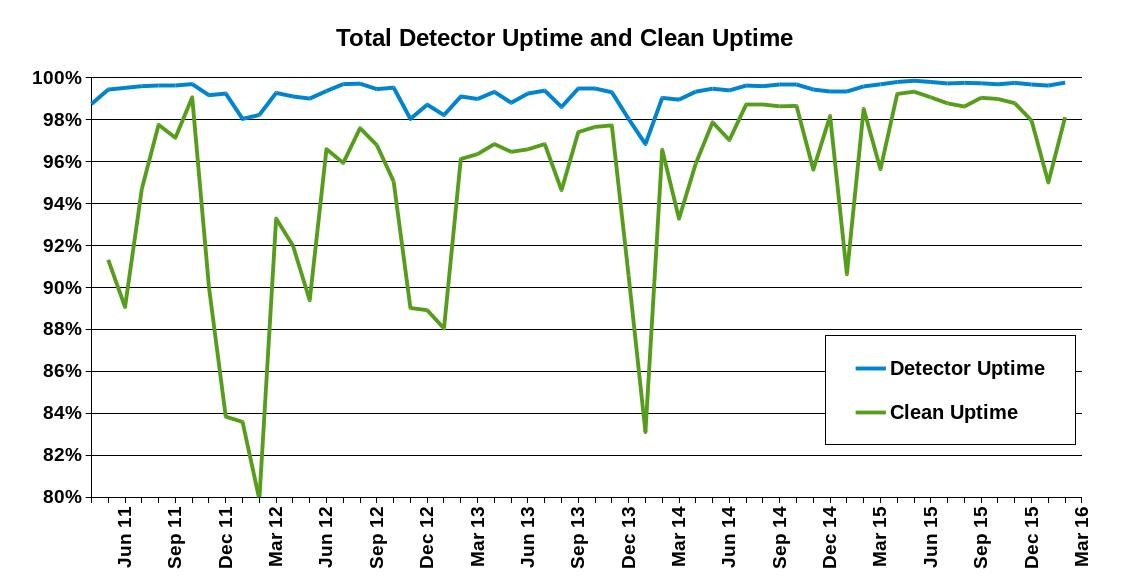
\includegraphics[width=0.8\textwidth]{graphics/uptime/uptime.jpg}
 \caption{Uptime of the IceCube detector.}
 \label{fig:uptime}
\end{figure}



